\section{Infanterietrupp / Fireteam (FT)}
\begin{wrapfigure}{R}{0.4\textwidth}
	\centering 
	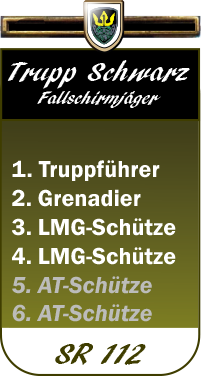
\includegraphics[width=0.3\textwidth]{./img/truppenordnung/infanterie/infanterie}
	%\caption{Beispiel eines Infantrietrupps}
\end{wrapfigure}
Die Infanterie bildet den Kernbestandteil vieler Missionen. Ein Infanterietrupp ist immer Teil eines Zuges und besteht aus 4 oder 6 Mann. Mögliche Positionen innerhalb eines Infanterietrupps sind:

	\begin{longtable}{p{0.4\linewidth}p{0.4\linewidth}}
		Truppführer (TF) & Fireteam Leader (FTL)\\
		\hline
		Grenadier (GRE) & \\
		\hline
		Leichter MG-Schütze (LMG) & Automatic Rifleman (AR)\\
		\hline
		Mittlerer MG-Schütze & Medium Machine Gunner (MMG) \\
		\hline
		MG-Assistent & Assistant Machine Gunner (AMG)\\ 
		& notwendig für MMG\\
		\hline
		Leichter Panzerabwehrschütze & Light Anti Tank (LAT)\\
		\hline	
		Schwerer Panzerabwehrschütze & Heavy Anti Tank (HAT)\\
		\hline	
		Panzerabwehr-Assistent & Assistant Anti Tank (AAT)\\ 
		& notwendig für HAT\\
		\hline	
		Luftabwehrschütze & Anti-Air (AA)\\
		\hline
		Pionier & Pioneer (PIO)\\
		\hline	
		Gefechtssanitäter & Combat Medic (CM)\\
		\hline				
		Schütze & Rifleman (RI)\\
		\hline									
	\end{longtable}

Auf eine sinnvolle Einteilung in Budd"=Teams (z.\,B. bei Positionen, die einen Assistenten erfordern), ist hierbei zu achten.\\
Die Kommunikation erfolgt ausschließlich über Short-Range, der Truppführer schaltet sich über seine Additional-Short-Range auf den Zugkanal auf, um sich mit der Zugführung und den anderen Truppführern im Zug abzusprechen. Die Nummer 2 im Trupp kann sich ebenfalls auf den Zugfunk aufschalten, jedoch nur mithören und nicht funken - es sei denn, der Truppführer fällt aus und die Nummer 2 übernimmt.